\documentclass[11pt]{amsart}

\usepackage[T1]{fontenc}
\usepackage{lmodern}
\usepackage{amssymb,amsmath}
\usepackage{booktabs,array}
\usepackage{graphicx}
\usepackage[dvipsnames]{xcolor}
\usepackage[margin=1.15in]{geometry}
\usepackage[colorlinks=true,linkcolor=blue!50!black,citecolor=blue!50!black,urlcolor=blue!50!black]{hyperref}

\newtheorem{theorem}{Theorem}[section]
\newtheorem{proposition}[theorem]{Proposition}
\newtheorem{lemma}[theorem]{Lemma}
\newtheorem{corollary}[theorem]{Corollary}
\theoremstyle{definition}
\newtheorem{definition}[theorem]{Definition}
\theoremstyle{remark}
\newtheorem{remark}[theorem]{Remark}

\numberwithin{equation}{section}
\numberwithin{table}{section}
\numberwithin{figure}{section}

\newcommand{\R}{\mathbb{R}}
\newcommand{\Z}{\mathbb{Z}}
\newcommand{\M}{\mathcal{M}}
\newcommand{\Rk}{\mathcal{R}}
\newcommand{\Sym}{\mathrm{Sym}}
\newcommand{\Min}{\operatorname{Min}}
\newcommand{\covol}{\operatorname{covol}}
\newcommand{\dist}{\operatorname{dist}}
\newcommand{\adj}{\operatorname{adj}}
\newcommand{\GL}{\mathrm{GL}}
\newcommand{\cand}{\mathcal{C}}
\hypersetup{pdftitle={Densest packings of two translates of a lattice in four dimensions},pdfauthor={Deep Bhattacharjee}}
\providecommand{\doi}[1]{\url{https://doi.org/#1}}

\begin{document}

\title[Packings of two lattice translates in four dimensions]{Densest packings of two translates\\ of a lattice in four dimensions}

\author{Deep Bhattacharjee}
\address{Formerly, Electro-Gravitational Space Propulsion Laboratory (EGSPL),\newline Bhubaneswar, Odisha 751030, India}
\email{d.bhattacharjee@erl-forschung.de}
\email{itsdeep@live.com}
\urladdr{https://orcid.org/0000-0003-0466-750X}
\thanks{Corresponding author: \href{mailto:d.bhattacharjee@erl-forschung.de}{d.bhattacharjee@erl-forschung.de}; ORCID \href{https://orcid.org/0000-0003-0466-750X}{\mbox{0000-0003-0466-750X}}}

\subjclass[2020]{Primary 52C17; Secondary 11H31, 11H55}
\keywords{sphere packing, periodic packing, $D_4$ lattice, $24$-cell, Voronoi cell, Ryshkov polyhedron}

\begin{abstract}
Let $\Lambda$ be a lattice in $\R^4$ and $b$ a vector outside $\Lambda$ such that any two distinct points of $\Lambda\cup(\Lambda+b)$ are at distance at least $2$. We prove that the covolume of $\Lambda$ is at least $16$, with equality only when $\Lambda\cup(\Lambda+b)$ is congruent to $\sqrt2\,D_4$. Thus no packing of unit balls whose centres form two translates of a lattice in $\R^4$ is denser than the $D_4$ lattice packing, and every Voronoi cell of such a packing has volume at least $8$, the volume of the regular $24$-cell, as Musin's $24$-cell conjecture predicts. The packing condition on the Gram matrix of a basis of $\Lambda$ together with $b$ cuts out a locally finite polyhedron. The concavity of $\log\det$ and of a Schur complement reduces the problem to the vertices and edges of this polyhedron. Up to integral symmetries it has ten vertices and $1137$ edges at them. This finite table is computed in exact arithmetic and re-checked by four independent programs; every other step is proved by hand.
\end{abstract}

\maketitle

\section{Introduction}

The root lattice $D_4=\{x\in\Z^4:x_1+x_2+x_3+x_4\in2\Z\}$, scaled by $\sqrt2$ so that its minimal distance is $2$, carries a packing of unit balls of density $\pi^2/16$. Korkine and Zolotarev proved that no lattice packing of balls in $\R^4$ is denser~\cite{KZ1877}. Whether $D_4$ is densest among all packings in $\R^4$ is open. Musin's $24$-cell conjecture~\cite{Musin2018} states that every Voronoi cell of a packing of unit balls in $\R^4$ has volume at least $8$, the volume of the regular $24$-cell, which is the Voronoi cell of $\sqrt2\,D_4$; it implies that $D_4$ is densest.

A periodic packing is a finite union of translates of one lattice. After lattices, the next case is two translates, $P=\Lambda\cup(\Lambda+b)$. Andreanov and Kallus~\cite{AK2020} extended Voronoi's algorithm for perfect forms~\cite{Voronoi1908} to such sets and enumerated the locally optimal ones in dimensions $3$, $4$ and $5$. In dimension $4$ their enumeration found $D_4$ densest. Parts of their computation used floating-point arithmetic, and they present these results as numerical rather than rigorous~\cite[\S4]{AK2020}. We prove the four-dimensional statement.

\begin{theorem}\label{thm:main}
Let $\Lambda\subset\R^4$ be a lattice and $b\in\R^4\setminus\Lambda$ such that $|x-y|\ge2$ for all distinct $x,y\in P=\Lambda\cup(\Lambda+b)$. Then $\covol(\Lambda)\ge16$, with equality if and only if $P$ is congruent to $\sqrt2\,D_4$. Equivalently, the packing of unit balls centred at the points of $P$ has density at most $\pi^2/16$, with equality only for $\sqrt2\,D_4$.
\end{theorem}

\begin{corollary}\label{cor:cells}
In a packing of unit balls in $\R^4$ whose centres form two translates of a lattice, every Voronoi cell has volume at least $8$. Equality holds only when the centres form $\sqrt2\,D_4$, and then every cell is a regular $24$-cell.
\end{corollary}

For a single lattice the bound of Corollary~\ref{cor:cells} is the theorem of Korkine and Zolotarev, so Corollary~\ref{cor:cells} proves the $24$-cell conjecture for all packings whose centres form at most two translates of a lattice.

\subsection*{Method}
A two-periodic set is encoded by the $5\times5$ Gram matrix $J$ of a basis of $\Lambda$ together with $b$. The packing condition becomes infinitely many linear inequalities $J[k]\ge4$, which cut out a locally finite polyhedron $\Rk$ (Section~\ref{sec:polyhedron}); packings are the points of $\Rk$ where $\det J=0$, and the quantity to minimise is $\det Q$, where $Q$ is the upper left $4\times4$ block of $J$. Proposition~\ref{prop:descent} shows that every packing can be moved, without increasing $\det Q$, to a vertex of $\Rk$ or to a point of an edge of $\Rk$. The argument uses only the concavity of $\log\det Q$ and of the Schur complement of $Q$ in $J$; it replaces the analysis of local optimality conditions and of ``fluid'' packings in~\cite[Theorem~3]{AK2020}.

Up to the integral symmetries of the problem, $\Rk$ has ten vertices and $1137$ edges at them (Proposition~\ref{prop:computation}). This is the one statement of the paper that rests on computation, which is finite and exact, and we give certificates that four independent programs re-check (Appendix~\ref{app:verification}). The ten vertices agree with~\cite{AK2020}. Everything else is proved by hand. The concavity of the Schur complement shows that bounded edges contain no packings in their interiors, and on the $25$ unbounded edges all quantities are explicit (Table~\ref{tab:unbounded}). The equality case uses a covering property of two sublattices of index two in $D_4$ (Lemma~\ref{lem:d4}).

The method is specific to two translates. Three or more translates, and the $24$-cell conjecture for arbitrary packings, are not treated here.

\section{Two-periodic sets and the polyhedron \texorpdfstring{$\Rk$}{R}}\label{sec:polyhedron}

\subsection{Notation}
$\Sym_n$ is the space of real symmetric $n\times n$ matrices, with any fixed norm $\|\cdot\|$. For $J\in\Sym_5$ and $x\in\R^5$ we write $J[x]=x^{\mathsf T}Jx$, and we write
\[
J=\begin{pmatrix}Q&r\\ r^{\mathsf T}&s\end{pmatrix},\qquad Q=Q(J)\in\Sym_4,\ r\in\R^4,\ s\in\R .
\]
Let $\M=\Z^4\times\{-1,0,1\}\subset\Z^5$ and $\M^*=\M\setminus\{0\}$. Elements of $\M$ are written $k=(n,l)$ with $n\in\Z^4$, $l\in\{-1,0,1\}$. Define
\[
\Rk=\{J\in\Sym_5:\ J[k]\ge4\ \text{for all }k\in\M^*\}.
\]
$\Rk$ is closed and convex. For $J\in\Rk$ let
\begin{gather*}
\Min(J)=\{k\in\M^*:J[k]=4\},\qquad C_J=\{X\in\Sym_5: X[k]\ge0\ \text{for all } k\in\Min(J)\},\\
L_J=C_J\cap(-C_J),
\end{gather*}
so $L_J=\{X:X[k]=0\ \forall k\in\Min(J)\}$, and let $d(J)=\dim L_J$. Since $k$ and $-k$ give the same condition, we list one vector of each pair $\pm k$ when counting $\Min(J)$.

Let $\Lambda\subset\R^4$ be a lattice with basis $a_1,\dots,a_4$ and $b\in\R^4$. The Gram matrix of $(a_1,\dots,a_4,b)$ is denoted $J(a,b)$. Then
\begin{equation}\label{eq:J}
J(a,b)[(n,l)]=\Bigl|\sum_{i=1}^4 n_ia_i+lb\Bigr|^2 .
\end{equation}

\begin{lemma}\label{lem:packing}
Let $b\notin\Lambda$. The distinct points of $\Lambda\cup(\Lambda+b)$ are at distance at least $2$ if and only if $J(a,b)\in\Rk$.
\end{lemma}

\begin{proof}
Since $\Lambda$ and $\Lambda+b$ are disjoint, the differences of distinct points are the vectors of $(\Lambda\setminus0)\cup(\Lambda+b)\cup(\Lambda-b)$, that is, the vectors $\sum n_ia_i+lb$ with $(n,l)\in\M^*$. Apply~\eqref{eq:J}.
\end{proof}

\begin{lemma}\label{lem:pd}
For $J\in\Rk$ the block $Q(J)$ is positive definite.
\end{lemma}

\begin{proof}
We have $Q[n]=J[(n,0)]\ge4$ for $n\in\Z^4\setminus0$. If $Q[x]<0$ for some $x\in\R^4$, the open cone $\{Q<0\}$ contains a rational point and hence an integral point $n\ne0$ with $Q[n]<0$, a contradiction. So $Q$ is positive semidefinite. Suppose $Qv=0$ with $\max_i|v_i|=1$. By Dirichlet's theorem on simultaneous approximation, for every integer $N\ge1$ there are an integer $1\le m\le N^4$ and $n\in\Z^4$ with $\max_i|mv_i-n_i|\le1/N$. Then $n\ne0$ because $\max_i|mv_i|=m\ge1>1/N$, and $Q[n]=Q[n-mv]\le16\|Q\|_{\infty}/N^2$, where $\|Q\|_\infty$ is the largest absolute value of an entry. For large $N$ this is less than $4$, a contradiction. Hence $Q$ is positive definite.
\end{proof}

Let $\Sym_5^+=\{J\in\Sym_5:Q(J)\text{ positive definite}\}$, an open convex set containing $\Rk$. For $J\in\Sym_5^+$ put
\[
q(J)=Q^{-1}r,\qquad \sigma(J)=s-r^{\mathsf T}Q^{-1}r .
\]

\begin{lemma}\label{lem:sigma}
Let $J\in\Sym_5^+$.
\begin{enumerate}
\item $J[(x,l)]=Q[x+l\,q(J)]+l^2\sigma(J)$ for $x\in\R^4$ and $l\in\R$.
\item $\sigma(J)=\min_{x\in\R^4}J[(x,1)]$, attained at $x=-q(J)$. In particular $\sigma(J')\le J'[u]$ for every $J'\in\Sym_5^+$ and every $u\in\R^4\times\{1\}$, and $\sigma$ is concave on $\Sym_5^+$.
\item $\det J=\det Q\cdot\sigma(J)$.
\end{enumerate}
\end{lemma}

\begin{proof}
(1) is completing the square, (2) follows from (1) because $Q$ is positive definite, and a minimum of affine functions of $J$ is concave. (3) is the Schur complement formula.
\end{proof}

\begin{lemma}\label{lem:rank4}
Let $J\in\Rk$.
\begin{enumerate}
\item $\sigma(J)=0$ if and only if $J=J(a,b)$ for a basis $a$ of a lattice $\Lambda$ and a vector $b\notin\Lambda$ such that the distinct points of $\Lambda\cup(\Lambda+b)$ are at distance at least $2$. In that case $\det Q(J)=\covol(\Lambda)^2$.
\item If $\sigma(J)<0$, then $J+|\sigma(J)|\,e_5e_5^{\mathsf T}\in\Rk$, its $Q$-block is $Q(J)$, and its $\sigma$ is $0$.
\end{enumerate}
\end{lemma}

\begin{proof}
(1) If $\sigma(J)=0$, then $J$ is positive semidefinite of rank $4$ by Lemma~\ref{lem:sigma}(1), (3) and Lemma~\ref{lem:pd}, hence the Gram matrix of five vectors $a_1,\dots,a_4,b$ of $\R^4$, and $a_1,\dots,a_4$ are linearly independent because $Q$ is positive definite. If $b$ were $\sum n_ia_i$, then $J[(-n,1)]=0<4$. Lemma~\ref{lem:packing} gives the packing property. Conversely $J(a,b)$ is a Gram matrix of five vectors in $\R^4$, so $\det J(a,b)=0$ and $\sigma=0$ by Lemma~\ref{lem:sigma}(3). Finally $\det Q=\det(a_i\cdot a_j)=\covol(\Lambda)^2$.
(2) Adding $|\sigma|e_5e_5^{\mathsf T}$ changes $J[(n,l)]$ by $l^2|\sigma|\ge0$, leaves $Q$ and $r$ unchanged and raises $s$, hence $\sigma$, by $|\sigma|$.
\end{proof}

\begin{lemma}\label{lem:minkowski}
For $J\in\Rk$, $\det Q(J)\ge\pi^4/4$.
\end{lemma}

\begin{proof}
$Q$ is the Gram matrix of a lattice $\Lambda$ with no nonzero vector of length less than $2$. The open ball of radius $2$ in $\R^4$ has volume $8\pi^2$. By Minkowski's convex body theorem~\cite[Ch.~III]{Cassels1959} it contains a nonzero point of $\Lambda$ if $8\pi^2>2^4\covol(\Lambda)$. Hence $\covol(\Lambda)\ge\pi^2/2$.
\end{proof}

\subsection{Local structure}

\begin{lemma}\label{lem:local}
\begin{enumerate}
\item For every compact set $K\subset\Sym_5^+$ the set $\M_K=\{k\in\M^*: J[k]\le5\text{ for some }J\in K\}$ is finite.
\item For every $J\in\Rk$ there is $\varepsilon>0$ such that for all $X\in\Sym_5$ with $\|X\|\le\varepsilon$ we have $J+X\in\Rk$ if and only if $X\in C_J$.
\item For every $J\in\Rk$, $\Min(J)$ is finite and $\Rk\subseteq J+C_J$.
\end{enumerate}
\end{lemma}

\begin{proof}
(1) On $K$ the smallest eigenvalue of $Q$ is at least some $\mu>0$, and $|q(J)|\le\rho$, $|\sigma(J)|\le\rho$ for some $\rho$, by continuity. For $k=(n,l)\in\M^*$ and $J\in K$, Lemma~\ref{lem:sigma}(1) gives $J[k]\ge\mu|n+lq(J)|^2-\rho$. If $|n|>\rho+\sqrt{(5+\rho)/\mu}$, then $|n+lq(J)|\ge|n|-\rho$ and $J[k]>5$.
(2) Choose $\varepsilon_0>0$ such that the closed ball $K=\bar B(J,\varepsilon_0)$ lies in $\Sym_5^+$. The finitely many $k\in\M_K\setminus\Min(J)$ have $J[k]>4$, so there is $\varepsilon\le\varepsilon_0$ with $(J+X)[k]>4$ for all of them whenever $\|X\|\le\varepsilon$. For such $X$, the vectors $k\notin\M_K$ satisfy $(J+X)[k]>5$, so $J+X\in\Rk$ if and only if $(J+X)[k]=4+X[k]\ge4$ for all $k\in\Min(J)$.
(3) $\Min(J)\subseteq\M_{\{J\}}$ is finite. If $J'\in\Rk$, then $J+\lambda(J'-J)\in\Rk$ for $\lambda\in[0,1]$, and by (2) $\lambda(J'-J)\in C_J$ for small $\lambda>0$; $C_J$ is a cone.
\end{proof}

\begin{lemma}\label{lem:nolines}
$\Rk$ contains no line.
\end{lemma}

\begin{proof}
If $J+\tau X\in\Rk$ for all $\tau\in\R$, then $X[k]=0$ for every $k\in\M^*$. The matrices $kk^{\mathsf T}$ for $k=e_i$ $(1\le i\le5)$ and $k=e_i+e_j$ $(1\le i<j\le5)$, all in $\M^*$, span $\Sym_5$, so $X=0$.
\end{proof}

\begin{definition}
A \emph{vertex} of $\Rk$ is a point $J\in\Rk$ with $d(J)=0$. Then $C_J$ is a pointed polyhedral cone, defined by the finitely many inequalities $X[k]\ge0$, $k\in\Min(J)$, whose linear forms span the $15$-dimensional dual of $\Sym_5$. An \emph{extreme ray} of $C_J$ is a ray $\R_{\ge0}Y$, $Y\ne0$, with $Y\in C_J$ such that $\{k\in\Min(J):Y[k]=0\}$ has rank $14$, i.e.\ the forms $X\mapsto X[k]$ for these $k$ span a $14$-dimensional space. For an extreme ray $Y$ put
\[
t^*(J,Y)=\sup\{t\ge0:J+tY\in\Rk\}\in(0,\infty],
\]
which is positive by Lemma~\ref{lem:local}(2). The set $\{J+tY:0\le t\le t^*\}$ (with $t<\infty$) is the \emph{edge} of $\Rk$ at $J$ in direction $Y$; it is \emph{bounded} if $t^*<\infty$.
\end{definition}

We use two standard facts on polyhedral cones~\cite[Lecture~1]{Ziegler1995}: a pointed polyhedral cone has finitely many extreme rays and is their conical hull, and a nonzero vector of the cone spans an extreme ray exactly when the inequalities it satisfies with equality have rank one less than the dimension.

\begin{lemma}\label{lem:edges}
Let $J$ be a vertex and $Y$ an extreme ray of $C_J$.
\begin{enumerate}
\item $\{t\ge0:J+tY\in\Rk\}$ is the interval $[0,t^*]$, or $[0,\infty)$ if $t^*=\infty$. If $t^*<\infty$, then $J+t^*Y$ is a vertex.
\item Every $J'\in\Rk$ with $d(J')=1$ lies on an edge: $J'=J_v+tY'$ for a vertex $J_v$, an extreme ray $Y'$ of $C_{J_v}$, and $0<t<t^*(J_v,Y')$.
\end{enumerate}
\end{lemma}

\begin{proof}
(1) The set is convex and closed. Let $J_1=J+t^*Y$ with $t^*<\infty$ and $Z=\{k\in\Min(J):Y[k]=0\}$. Every $k\in Z$ has $J_1[k]=4$, so $Z\subseteq\Min(J_1)$. Since $J_1+\eta Y\notin\Rk$ for $\eta>0$, Lemma~\ref{lem:local}(2) gives $Y\notin C_{J_1}$, so some $k_1\in\Min(J_1)$ has $Y[k_1]<0$. The forms of $Z$ vanish on $Y$ and span a $14$-dimensional space, and the form of $k_1$ does not vanish on $Y$; together they have rank $15$, so $L_{J_1}=0$.
(2) Let $L_{J'}=\R X_0$. The set $I_0=\{\tau:J'+\tau X_0\in\Rk\}$ is a closed interval which contains a neighbourhood of $0$ by Lemma~\ref{lem:local}(2) and is not $\R$ by Lemma~\ref{lem:nolines}. Let $\tau_e$ be a finite end point, $J_v=J'+\tau_eX_0$ and $Y'=-\operatorname{sgn}(\tau_e)X_0$. Since $X_0[k]=0$ for $k\in\Min(J')$, we have $\Min(J')\subseteq\Min(J_v)$ and $L_{J_v}\subseteq L_{J'}$. If $X_0\in L_{J_v}$, then $J_v\pm\eta X_0\in\Rk$ for small $\eta$ by Lemma~\ref{lem:local}(2), contradicting the choice of $\tau_e$; so $d(J_v)=0$. The segment from $J_v$ to $J'$ lies in $\Rk$, so $Y'\in C_{J_v}$ by Lemma~\ref{lem:local}(2), and $Y'$ vanishes on $\Min(J')$, which has rank $14$; so $Y'$ spans an extreme ray of $C_{J_v}$, and $J'=J_v+|\tau_e|Y'$. Finally $|\tau_e|<t^*(J_v,Y')$, since otherwise $J'$ would be a vertex by (1).
\end{proof}

\subsection{Symmetries}
Let $\Gamma$ be the group of matrices
\[
T=\begin{pmatrix}U&v\\0&\varepsilon\end{pmatrix},\qquad U\in\GL_4(\Z),\ v\in\Z^4,\ \varepsilon\in\{1,-1\}.
\]
Then $T(n,l)=(Un+lv,\varepsilon l)$, so $T$ maps $\M$ bijectively onto itself, and $J\mapsto T^{\mathsf T}JT$ maps $\Rk$ bijectively onto itself with $(T^{\mathsf T}JT)[k]=J[Tk]$. Consequently $\Min(T^{\mathsf T}JT)=T^{-1}\Min(J)$, $X\mapsto T^{\mathsf T}XT$ maps $C_J$ onto $C_{T^{\mathsf T}JT}$, and vertices, extreme rays, edges and the values $t^*$ correspond. Moreover $Q(T^{\mathsf T}JT)=U^{\mathsf T}QU$, so $\det Q$, $\det J$ and $\sigma=\det J/\det Q$ are $\Gamma$-invariant. In terms of point sets, $T$ replaces the basis $a$ by $aU$ and $b$ by $\varepsilon b+\sum v_ia_i$, so $J(a,b)$ and $T^{\mathsf T}J(a,b)T$ describe congruent sets. We call $J,J'$ \emph{equivalent} if $J'=T^{\mathsf T}JT$ for some $T\in\Gamma$.

\subsection{Reaching all vertices}

\begin{proposition}\label{prop:connected}
Let $v$ and $w$ be vertices of $\Rk$. There are vertices $v=v_0,v_1,\dots,v_m=w$ such that $v_{s+1}=v_s+t^*Y_s$ for an extreme ray $Y_s$ of $C_{v_s}$ with $t^*(v_s,Y_s)<\infty$.
\end{proposition}

\begin{proof}
Let $\ell(X)=\sum_{k\in\Min(w)}X[k]$. Then $\ell\ge0$ on $C_w$, and $\ell(X)=0$ for $X\in C_w$ only if $X\in L_w=0$. By compactness of $\{X\in C_w:\|X\|=1\}$ there is $\delta>0$ with $\ell(X)\ge\delta\|X\|$ on $C_w$. By Lemma~\ref{lem:local}(3), $\Rk\subseteq w+C_w$, so $\ell(J)>\ell(w)$ for $J\in\Rk\setminus\{w\}$, and for every $c$ the set $S_c=\{J\in\Rk:\ell(J)\le c\}$ is compact. A vertex $J$ is the unique solution of the linear equations $J[k]=4$, $k\in\Min(J)$, and the vertices in $S_c$ have $\Min(J)\subseteq\M_{S_c}$, a finite set by Lemma~\ref{lem:local}(1) (note $S_c\subset\Rk\subset\Sym_5^+$). So $S_c$ contains finitely many vertices.

Let $u$ be a vertex with $u\ne w$. If $\ell(Y)\ge0$ for every extreme ray of $C_u$, then $\ell\ge0$ on $C_u$, and $\Rk\subseteq u+C_u$ gives $\ell(w)\ge\ell(u)$, which is false. So some extreme ray $Y$ of $C_u$ has $\ell(Y)<0$. Along $u+tY$ the value of $\ell$ decreases, and $S_{\ell(u)}$ is compact, so $t^*(u,Y)<\infty$, and $u'=u+t^*Y$ is a vertex (Lemma~\ref{lem:edges}) with $\ell(u')<\ell(u)$. Starting from $u=v$ and repeating, we obtain a sequence of vertices in $S_{\ell(v)}$ along which $\ell$ strictly decreases. It is finite, and it can only stop at $w$.
\end{proof}

\begin{corollary}\label{cor:closure}
Let $J_0,\dots,J_N$ be vertices of $\Rk$ such that for every $i$ and every extreme ray $Y$ of $C_{J_i}$ with $t^*(J_i,Y)<\infty$ the vertex $J_i+t^*Y$ is equivalent to some $J_j$. Then every vertex of $\Rk$ is equivalent to some $J_j$, and every edge of $\Rk$ is equivalent to an edge at some $J_j$.
\end{corollary}

\begin{proof}
Let $w$ be a vertex and take the path $J_0=v_0,\dots,v_m=w$ of Proposition~\ref{prop:connected}. If $v_s=T^{\mathsf T}J_iT$, then $Y'=T^{-\mathsf T}Y_sT^{-1}$ is an extreme ray of $C_{J_i}$ with the same $t^*$, and $v_{s+1}=T^{\mathsf T}(J_i+t^*Y')T$, which is equivalent to some $J_j$ by hypothesis. By induction $w$ is equivalent to some $J_j$. An edge at a vertex $w=T^{\mathsf T}J_jT$ in direction $Y$ is the image under $T$ of the edge at $J_j$ in direction $T^{-\mathsf T}YT^{-1}$.
\end{proof}

\section{Reduction to vertices and edges}\label{sec:reduction}

\begin{lemma}\label{lem:logdet}
Let $Q$ be positive definite and $H\in\Sym_4$, $H\ne0$. On the open interval of $\tau$ where $Q+\tau H$ is positive definite, $\psi(\tau)=\log\det(Q+\tau H)$ is strictly concave.
\end{lemma}

\begin{proof}
With $Q_\tau=Q+\tau H$ we have $\psi'(\tau)=\operatorname{tr}(Q_\tau^{-1}H)$ and $\psi''(\tau)=-\operatorname{tr}\bigl((Q_\tau^{-1/2}HQ_\tau^{-1/2})^2\bigr)<0$, because $Q_\tau^{-1/2}HQ_\tau^{-1/2}$ is a nonzero symmetric matrix.
\end{proof}

Let
\[
S=\{J\in\Rk:\sigma(J)\le0\},\qquad
\cand=\{J\in S: d(J)=0\}\ \cup\ \{J\in\Rk: d(J)=1,\ \sigma(J)=0\}.
\]
So $\cand$ consists of the vertices with $\det J\le0$ and of the points with $\det J=0$ in the relative interiors of edges. By Lemma~\ref{lem:rank4}, the infimum of $\det Q$ over $S$ equals the infimum of $\covol(\Lambda)^2$ over the sets of Theorem~\ref{thm:main}.

\begin{proposition}\label{prop:descent}
For every $J\in S$ there is $J'\in\cand$ with $\det Q(J')\le\det Q(J)$. If $\det Q(J)=\inf_S\det Q$, then $J'$ can be chosen with $Q(J')=Q(J)$.
\end{proposition}

\begin{proof}
Write $f(J)=\log\det Q(J)$ and $\pi(J)=2d(J)+[\sigma(J)<0]$, where $[\cdot]$ is $1$ if the condition holds and $0$ otherwise. We show: if $J\in S\setminus\cand$, there is $J_1\in S$ with $f(J_1)\le f(J)$ and $\pi(J_1)<\pi(J)$, and $Q(J_1)=Q(J)$ if $f(J)=\inf_Sf$. Induction on $\pi$ then proves the proposition.

Let $J\in S\setminus\cand$. Then either (a) $\sigma(J)<0$ and $d(J)\ge1$, or (b) $\sigma(J)=0$ and $d(J)\ge2$. In case (a) choose any $X\in L_J\setminus0$. In case (b) let $u=(-q(J),1)\in\R^5$, so that $J[u]=\sigma(J)=0$ by Lemma~\ref{lem:sigma}(2), and choose $X\in L_J\setminus0$ with $X[u]=0$, which exists because $\dim L_J\ge2$. Put $J(\tau)=J+\tau X$ and
\[
I_0=\{\tau\in\R:J(\tau)\in\Rk\}.
\]
$I_0$ is a closed interval, it contains a neighbourhood of $0$ by Lemma~\ref{lem:local}(2) because $\pm X\in C_J$, and $I_0\ne\R$ by Lemma~\ref{lem:nolines}. Since $X[k]=0$ for $k\in\Min(J)$, we have $J(\tau)[k]=4$ for these $k$, hence
\begin{equation}\label{eq:mininc}
\Min(J)\subseteq\Min(J(\tau))\quad\text{and}\quad L_{J(\tau)}\subseteq L_J\qquad(\tau\in I_0).
\end{equation}
In case (b), Lemma~\ref{lem:sigma}(2) gives $\sigma(J(\tau))\le J(\tau)[u]=J[u]+\tau X[u]=0$ for $\tau\in I_0$, and we put $I=I_0$. In case (a), $\tau\mapsto\sigma(J(\tau))$ is continuous on $I_0$ and negative at $0$, and we let $I$ be the connected component of $\{\tau\in I_0:\sigma(J(\tau))\le0\}$ containing $0$. In both cases $I$ is a closed interval, $0$ is an interior point of $I$, $I\ne\R$, and $J(\tau)\in S$ for $\tau\in I$.

The function $\varphi(\tau)=f(J(\tau))$ is concave on $I$ by Lemma~\ref{lem:logdet} (it is constant if $Q(X)=0$), and bounded below by Lemma~\ref{lem:minkowski}. If $I=[\alpha,\beta]$ is bounded, concavity gives $\varphi(0)\ge\min(\varphi(\alpha),\varphi(\beta))$. If $I=[\alpha,\infty)$, then $\varphi$ is nondecreasing, because a concave function that decreases somewhere on a half-line tends to $-\infty$; so $\varphi(\alpha)\le\varphi(0)$, and similarly for $I=(-\infty,\beta]$. In every case there is a finite end point $\tau_0$ of $I$ with $\varphi(\tau_0)\le\varphi(0)$. Put $J_1=J(\tau_0)$. Then $J_1\in S$ and $f(J_1)\le f(J)$.

If $\tau_0$ is an end point of $I_0$, then $X\notin L_{J_1}$: otherwise $J_1\pm\eta X\in\Rk$ for small $\eta>0$ by Lemma~\ref{lem:local}(2). With~\eqref{eq:mininc}, $d(J_1)\le d(J)-1$ and $\pi(J_1)\le2d(J)-1<\pi(J)$. If $\tau_0$ is not an end point of $I_0$, we are in case (a), $\sigma(J_1)=0$ by the choice of $I$, and $\pi(J_1)=2d(J_1)\le2d(J)<\pi(J)$.

Now let $f(J)=m:=\inf_Sf$. Then $\varphi\ge m$ on $I$ and $\varphi(0)=m$. Let $\tau_1$ lie strictly between $0$ and $\tau_0$, and let $\tau'\in I$ lie on the other side of $0$. Writing $0=\lambda\tau'+(1-\lambda)\tau_1$ with $0<\lambda<1$, concavity gives $m\ge\lambda\varphi(\tau')+(1-\lambda)\varphi(\tau_1)\ge\lambda m+(1-\lambda)\varphi(\tau_1)$, so $\varphi(\tau_1)\le m$, hence $\varphi(\tau_1)=m$. Thus $\varphi$ is constant on the nondegenerate interval between $0$ and $\tau_0$, Lemma~\ref{lem:logdet} forces $Q(X)=0$, and $Q(J_1)=Q(J)$. Also $f(J_1)=m$, so the induction carries the equality case along.
\end{proof}

\begin{figure}[t]
\centering
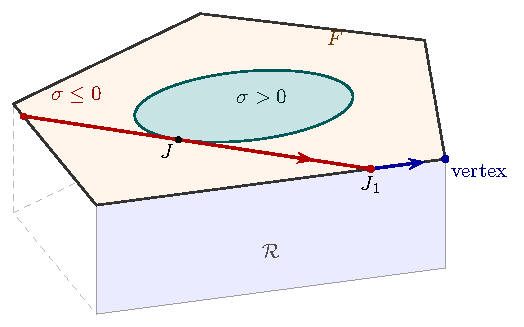
\includegraphics[width=0.78\textwidth]{figures/descent}
\caption{One step of the proof of Proposition~\ref{prop:descent} in a two-dimensional face $F$ of $\Rk$, the case $\sigma(J)=0$. The set $F\cap\{\sigma>0\}$ (shaded) is convex because $\sigma$ is concave. On the line through $J$ in the direction $X$, chosen with $X[u]=0$, we have $\sigma\le0$, and $\log\det Q$ is concave on it, so one of the two ends of the chord, here $J_1$, has $\det Q(J_1)\le\det Q(J)$. The point $J_1$ lies on an edge of $F$. From there the same step moves along the edge to a vertex or to a point with $\sigma=0$.}
\label{fig:descent}
\end{figure}

\section{Two sublattices of index two in \texorpdfstring{$D_4$}{D4}}\label{sec:d4}

For $n\ge2$ let $D_n=\{x\in\Z^n:\sum x_i\in2\Z\}$. In $D_4$ consider the sublattices of index two
\[
\Lambda_1=\{x\in D_4:x_1\in2\Z\}=2\Z\oplus D_3,\qquad \Lambda_2=\{x\in D_4:x_1+x_2\in2\Z\}=D_2\oplus D_2,
\]
where $D_2\oplus D_2$ refers to the coordinate pairs $(x_1,x_2)$ and $(x_3,x_4)$.

\begin{lemma}\label{lem:dn}
Let $n\in\{2,3\}$. For every $z\in\R^n$, $\dist(z,D_n)\le1$, with equality if and only if $z\in\Z^n\setminus D_n$. For every $t\in\R$, $\dist(t,2\Z)\le1$, with equality if and only if $t$ is an odd integer.
\end{lemma}

\begin{proof}
The second statement is clear. Let $m\in\Z^n$ with $|z_i-m_i|\le\frac12$ for all $i$. If $m\in D_n$, then $\dist(z,D_n)^2\le n/4<1$. Otherwise let $\delta=\max_i|z_i-m_i|$, attained at $i$, and let $m'=m+\epsilon e_i$ with $\epsilon=1$ if $z_i\ge m_i$ and $\epsilon=-1$ otherwise. Then $m'\in D_n$ and
\[
|z-m'|^2=|z-m|^2-\delta^2+(1-\delta)^2\le n\delta^2-2\delta+1 .
\]
Since $0\le\delta\le\frac12<\frac2n$, this is at most $1$, with equality only for $\delta=0$, that is $z=m\in\Z^n\setminus D_n$. Conversely, for $z\in\Z^n\setminus D_n$ and $x\in D_n$ the vector $x-z$ is integral with odd coordinate sum, so $|x-z|\ge1$.
\end{proof}

\begin{lemma}\label{lem:d4}
For $i\in\{1,2\}$ and every $y\in\R^4$, $\dist(y,\Lambda_i)\le\sqrt2$, with equality if and only if $y\in D_4\setminus\Lambda_i$.
\end{lemma}

\begin{proof}
The sums are orthogonal. For $\Lambda_1$, $\dist(y,\Lambda_1)^2=\dist(y_1,2\Z)^2+\dist((y_2,y_3,y_4),D_3)^2\le2$, with equality if and only if $y_1$ is odd and $(y_2,y_3,y_4)\in\Z^3\setminus D_3$ (Lemma~\ref{lem:dn}), that is, $y\in\Z^4$, $y_1$ odd and $\sum y_i$ even, which means $y\in D_4\setminus\Lambda_1$. For $\Lambda_2$, $\dist(y,\Lambda_2)^2=\dist((y_1,y_2),D_2)^2+\dist((y_3,y_4),D_2)^2\le2$, with equality if and only if $y\in\Z^4$ with $y_1+y_2$ and $y_3+y_4$ odd, which means $y\in D_4\setminus\Lambda_2$.
\end{proof}

\begin{corollary}\label{cor:d4}
Let $\Lambda=\phi(\sqrt2\,\Lambda_i)$ for a linear isometry $\phi$ of $\R^4$ and $i\in\{1,2\}$. If $\dist(b,\Lambda)\ge2$, then $\Lambda\cup(\Lambda+b)=\phi(\sqrt2\,D_4)$.
\end{corollary}

\begin{proof}
$y=\phi^{-1}(b)/\sqrt2$ has $\dist(y,\Lambda_i)\ge\sqrt2$, so $y\in D_4\setminus\Lambda_i$ by Lemma~\ref{lem:d4}. As $[D_4:\Lambda_i]=2$, $D_4=\Lambda_i\cup(\Lambda_i+y)$; apply $\sqrt2\,\phi$.
\end{proof}

The lattices $\sqrt2\,\Lambda_2$ and $\sqrt2\,\Lambda_1$ have the Gram matrices
\begin{equation}\label{eq:grams}
G_2=4I_4\quad\text{(basis }\sqrt2(e_1\pm e_2),\ \sqrt2(e_3\pm e_4)\text{)},\qquad
G_1=\begin{pmatrix}8&0&0&0\\0&4&2&2\\0&2&4&2\\0&2&2&4\end{pmatrix}
\end{equation}
(basis $2\sqrt2\,e_1$, $\sqrt2(e_2+e_3)$, $\sqrt2(e_2+e_4)$, $\sqrt2(e_3+e_4)$; here $e_2+e_3$, $e_2+e_4$, $e_3+e_4$ lie in $D_3$ and have determinant $\pm2=[\Z^3:D_3]$, so they form a basis of $D_3$). Both have determinant $256$.

\section{The vertices and edges of \texorpdfstring{$\Rk$}{R}}\label{sec:computation}

\begin{table}[t]
\centering
\small
\renewcommand{\arraystretch}{1.0}
\begin{tabular}{@{}c c c c c c c c@{}}
\toprule
$i$ & $J_i$ & $|\Min(J_i)|$ & $\det Q$ & $\det J$ & $|\Gamma_{J_i}|$ & rays & orbits\\
\midrule
0 & $\vphantom{\rule[-19pt]{0pt}{42pt}}\left(\begin{smallmatrix}4&0&0&0&2\\0&4&0&0&-2\\0&0&4&0&-2\\0&0&0&4&-2\\2&-2&-2&-2&4\end{smallmatrix}\right)$ & 20 & 256 & 0 & 768 & 60 & 4\\
1 & $\vphantom{\rule[-19pt]{0pt}{42pt}}\left(\begin{smallmatrix}4&0&0&0&2\\0&4&2&2&-4\\0&2&4&2&-4\\0&2&2&4&-4\\2&-4&-4&-4&8\end{smallmatrix}\right)$ & 19 & 128 & 128 & 192 & 169 & 11\\
2 & $\vphantom{\rule[-19pt]{0pt}{42pt}}\left(\begin{smallmatrix}4&0&0&0&2\\0&4&0&0&-2\\0&0&4&2&-2\\0&0&2&4&-2\\2&-2&-2&-2&4\end{smallmatrix}\right)$ & 17 & 192 & 128 & 96 & 33 & 5\\
3 & $\vphantom{\rule[-19pt]{0pt}{42pt}}\left(\begin{smallmatrix}4&-2&-2&-2&6\\-2&4&2&2&-6\\-2&2&4&2&-6\\-2&2&2&4&-6\\6&-6&-6&-6&16\end{smallmatrix}\right)$ & 20 & 80 & 128 & 240 & 400 & 16\\
4 & $\vphantom{\rule[-19pt]{0pt}{42pt}}\left(\begin{smallmatrix}4&0&-2&2&2\\0&4&2&2&-4\\-2&2&4&0&-4\\2&2&0&4&-2\\2&-4&-4&-2&8\end{smallmatrix}\right)$ & 20 & 64 & 128 & 768 & 400 & 9\\
5 & $\vphantom{\rule[-19pt]{0pt}{42pt}}\left(\begin{smallmatrix}4&0&-1&1&2\\0&6&3&3&-6\\-1&3&4&2&-5\\1&3&2&4&-4\\2&-6&-5&-4&10\end{smallmatrix}\right)$ & 15 & 108 & 162 & 96 & 15 & 3\\
6 & $\vphantom{\rule[-19pt]{0pt}{42pt}}\left(\begin{smallmatrix}4&0&0&0&2\\0&4&2&2&-4\\0&2&4&0&-2\\0&2&0&4&-4\\2&-4&-2&-4&8\end{smallmatrix}\right)$ & 15 & 128 & 192 & 96 & 15 & 3\\
7 & $\vphantom{\rule[-19pt]{0pt}{42pt}}\left(\begin{smallmatrix}4&-2&0&0&2\\-2&4&0&0&-2\\0&0&4&2&-2\\0&0&2&4&-2\\2&-2&-2&-2&4\end{smallmatrix}\right)$ & 15 & 144 & 192 & 144 & 15 & 2\\
8 & $\vphantom{\rule[-19pt]{0pt}{42pt}}\left(\begin{smallmatrix}6&-3&-3&-3&9\\-3&4&2&1&-6\\-3&2&4&2&-6\\-3&1&2&4&-6\\9&-6&-6&-6&18\end{smallmatrix}\right)$ & 15 & 81 & 162 & 144 & 15 & 2\\
9 & $\vphantom{\rule[-19pt]{0pt}{42pt}}\left(\begin{smallmatrix}4&-2&-2&-2&6\\-2&4&2&2&-6\\-2&2&4&2&-4\\-2&2&2&4&-6\\6&-6&-4&-6&16\end{smallmatrix}\right)$ & 15 & 80 & 192 & 240 & 15 & 2\\
\bottomrule
\end{tabular}
\caption{The ten vertices $J_i$ of $\Rk$ up to equivalence. $|\Min(J_i)|$ counts pairs $\pm k$; $\Gamma_{J_i}$ is the stabiliser of $J_i$ in $\Gamma$; ``rays'' is the number of extreme rays of $C_{J_i}$ and ``orbits'' the number of their orbits under $\Gamma_{J_i}$. The pairs $(\det Q,\det J)$ are distinct, so no two $J_i$ are equivalent.}
\label{tab:vertices}
\end{table}

\begin{table}[t]
\centering
\small
\renewcommand{\arraystretch}{1.2}
\begin{tabular}{@{}c l@{}}
\toprule
$i$ & end points of the edges at $J_i$: class $j$ of $J_i+t^*Y$, with $t^*$, and number of edges (orbits)\\
\midrule
0 & $1\,(2){:}\,16\,(1)$;\ $2\,(2){:}\,24\,(1)$;\ $3\,(2){:}\,16\,(1)$;\ $\infty{:}\,4\,(1)$\\
1 & $0\,(2){:}\,4\,(1)$;\ $1\,(2){:}\,36\,(2)$;\ $2\,(2){:}\,24\,(1)$;\ $3\,(2){:}\,64\,(2)$;\ $4\,(2){:}\,12\,(1)$;\ $5\,(1){:}\,12\,(1)$;\ $6\,(2){:}\,12\,(1)$;\ $\infty{:}\,5\,(2)$\\
2 & $0\,(2){:}\,3\,(1)$;\ $1\,(2){:}\,12\,(1)$;\ $3\,(2){:}\,12\,(1)$;\ $7\,(2){:}\,4\,(1)$;\ $\infty{:}\,2\,(1)$\\
3 & $0\,(2){:}\,5\,(1)$;\ $1\,(2){:}\,80\,(2)$;\ $2\,(2){:}\,30\,(1)$;\ $3\,(2){:}\,155\,(4)$;\ $4\,(2){:}\,50\,(2)$;\ $5\,(1){:}\,20\,(1)$;\\
  & $6\,(2){:}\,20\,(1)$;\ $7\,(2){:}\,15\,(1)$;\ $8\,(1){:}\,15\,(1)$;\ $9\,(2){:}\,5\,(1)$;\ $\infty{:}\,5\,(1)$\\
4 & $1\,(2){:}\,48\,(1)$;\ $3\,(2){:}\,160\,(2)$;\ $4\,(2){:}\,112\,(2)$;\ $5\,(1){:}\,8\,(1)$;\ $8\,(1){:}\,32\,(1)$;\ $9\,(2){:}\,32\,(1)$;\ $\infty{:}\,8\,(1)$\\
5 & $1\,(1){:}\,6\,(1)$;\ $3\,(1){:}\,8\,(1)$;\ $4\,(1){:}\,1\,(1)$\\
6 & $1\,(2){:}\,6\,(1)$;\ $3\,(2){:}\,8\,(1)$;\ $\infty{:}\,1\,(1)$\\
7 & $2\,(2){:}\,6\,(1)$;\ $3\,(2){:}\,9\,(1)$\\
8 & $3\,(1){:}\,9\,(1)$;\ $4\,(1){:}\,6\,(1)$\\
9 & $3\,(2){:}\,5\,(1)$;\ $4\,(2){:}\,10\,(1)$\\
\bottomrule
\end{tabular}
\caption{The edges at the vertices $J_i$. An entry $j\,(t^*){:}\,N\,(o)$ means that $N$ extreme rays $Y$ of $C_{J_i}$, forming $o$ orbits under $\Gamma_{J_i}$, have $t^*(J_i,Y)=t^*$ and $J_i+t^*Y$ equivalent to $J_j$; the entry $\infty$ counts the unbounded edges. No edge joins two vertices of class $0$.}
\label{tab:edges}
\end{table}

\begin{proposition}\label{prop:computation}
The matrices $J_0,\dots,J_9$ of Table~\ref{tab:vertices} are vertices of $\Rk$ with the stated invariants, and their edges are as in Table~\ref{tab:edges}. In particular:
\begin{enumerate}
\item for every $i$ and every extreme ray $Y$ of $C_{J_i}$ with $t^*(J_i,Y)<\infty$, the vertex $J_i+t^*Y$ is equivalent to some $J_j$, and $(i,j)\ne(0,0)$;
\item every extreme ray $Y$ of $C_{J_i}$ with $t^*(J_i,Y)=\infty$ equals $X_{u,a}$ (Definition~\ref{def:Xua}) for some $u\in\Z^4$, $a\in\Z$, and is equivalent under $\Gamma_{J_i}$ to one of the seven rays in Table~\ref{tab:unbounded}.
\end{enumerate}
\end{proposition}

\begin{proof}
This is a finite computation in exact integer and rational arithmetic, described in Appendix~\ref{app:verification}. For each of the $1112$ bounded edges it produces $t^*$, the class $j$ and a matrix $T\in\Gamma$ with $T^{\mathsf T}J_jT=J_i+t^*Y$; for each of the $25$ unbounded edges it produces $(u,a)$. These certificates and the completeness of the lists of extreme rays are checked by independent programs.
\end{proof}

By Corollary~\ref{cor:closure} and Proposition~\ref{prop:computation}(1), every vertex of $\Rk$ is equivalent to exactly one $J_i$, and every edge of $\Rk$ is equivalent to an edge at some $J_i$.

\begin{definition}\label{def:Xua}
For $u\in\Z^4$ and $a\in\Z$ let $p=(u,-a)$, $q=(u,-a-1)\in\Z^5$ and $X_{u,a}=pq^{\mathsf T}+qp^{\mathsf T}$. Thus $Q(X_{u,a})=2uu^{\mathsf T}$ and
\[
X_{u,a}[(n,l)]=2\,(u\cdot n-al)\,(u\cdot n-(a+1)l).
\]
\end{definition}

\begin{lemma}\label{lem:Xua}
$X_{u,a}[k]\ge0$ for all $k\in\M$. Hence $J+tX_{u,a}\in\Rk$ for all $J\in\Rk$ and $t\ge0$, and
\[
\det Q(J+tX_{u,a})=\det Q(J)+2t\,\adj(Q(J))[u].
\]
\end{lemma}

\begin{proof}
For $k=(n,l)$ the two factors $u\cdot n-al$ and $u\cdot n-(a+1)l$ are integers that differ by $l\in\{-1,0,1\}$; two such integers have a nonnegative product. The determinant formula is the matrix determinant lemma for the rank-one update $Q+2t\,uu^{\mathsf T}$.
\end{proof}

\begin{table}[t]
\centering
\small
\renewcommand{\arraystretch}{1.25}
\begin{tabular}{@{}c c r c c c c@{}}
\toprule
$i$ & $(u,a)$ & $N$ & $\det Q(J_i+tX_{u,a})$ & $\det(J_i+tX_{u,a})$ & $t_0>0$ & $\det Q$ at $t_0$\\
\midrule
0 & $(e_1,-1)$ & 4 & $128(t+2)$ & $-64\,t(t+2)$ & none & ---\\
1 & $((0,1,1,1),1)$ & 4 & $32(3t+4)$ & $-16(t-2)(3t+4)$ & $2$ & $320$\\
1 & $(e_1,-1)$ & 1 & $64(t+2)$ & $-32(t-2)(t+2)$ & $2$ & $256$\\
2 & $(e_1,-1)$ & 2 & $96(t+2)$ & $-16(t+2)(3t-4)$ & $4/3$ & $320$\\
3 & $((1,-1,-1,-1),-3)$ & 5 & $16(4t+5)$ & $-32(t^2-2t-4)$ & $1+\sqrt5$ & $144+64\sqrt5$\\
4 & $(e_3,0)$ & 8 & $64(t+1)$ & $-32(t-4)(t+1)$ & $4$ & $320$\\
6 & $(e_1,-1)$ & 1 & $64(t+2)$ & $-32(t-3)(t+2)$ & $3$ & $320$\\
\bottomrule
\end{tabular}
\caption{The unbounded edges $J_i+tX_{u,a}$, $t\ge0$, one per orbit under $\Gamma_{J_i}$; $N$ is the size of the orbit. The last two columns give the positive root $t_0$ of $\det(J_i+tX_{u,a})$ and the value of $\det Q$ there. Each row is a direct computation (the $\det Q$ column by Lemma~\ref{lem:Xua}); $144+64\sqrt5\approx287.11$.}
\label{tab:unbounded}
\end{table}

\begin{proposition}\label{prop:candidates}
Every $J\in\cand$ is equivalent to $J_0$ or to $J_i+t_0X_{u,a}$ for a row of Table~\ref{tab:unbounded} with a root $t_0$. In particular $\det Q(J)\ge256$ for all $J\in\cand$, and $\det Q(J)=256$ only if $J$ is equivalent to $J_0$ or to $J_1+2X_{e_1,-1}$.
\end{proposition}

\begin{proof}
Let $J\in\cand$. If $d(J)=0$, then $J$ is equivalent to some $J_i$, and $\sigma(J)=\sigma(J_i)=\det J_i/\det Q(J_i)$. By Table~\ref{tab:vertices} this is positive unless $i=0$, and $J\in S$ requires $\sigma(J)\le0$; so $J$ is equivalent to $J_0$.

If $d(J)=1$ and $\sigma(J)=0$, Lemma~\ref{lem:edges}(2) places $J$ in the relative interior of an edge, and after applying an element of $\Gamma$ we may assume $J=J_i+tY$ with $Y$ an extreme ray of $C_{J_i}$ and $0<t<t^*(J_i,Y)$. Suppose $t^*<\infty$. By Proposition~\ref{prop:computation}(1) the end point $J_i+t^*Y$ is equivalent to some $J_j$ with $(i,j)\ne(0,0)$, so $\sigma\ge0$ at both end points and $\sigma>0$ at one of them. The segment lies in $\Rk\subset\Sym_5^+$, where $\sigma$ is concave (Lemma~\ref{lem:sigma}(2)), so
\[
\sigma(J_i+tY)\ \ge\ \Bigl(1-\frac t{t^*}\Bigr)\sigma(J_i)+\frac t{t^*}\,\sigma(J_i+t^*Y)\ >\ 0,
\]
a contradiction. Hence $t^*=\infty$. By Proposition~\ref{prop:computation}(2), after applying an element of $\Gamma_{J_i}$, $Y=X_{u,a}$ for a row of Table~\ref{tab:unbounded}, and $\sigma(J)=0$ means $\det(J_i+tX_{u,a})=0$ (Lemma~\ref{lem:sigma}(3)), so $t=t_0$. The values of $\det Q$ are read off Table~\ref{tab:unbounded} and Table~\ref{tab:vertices}.
\end{proof}

\section{Proofs of Theorem~\ref{thm:main} and Corollary~\ref{cor:cells}}\label{sec:proofs}

\begin{proof}[Proof of Theorem~\ref{thm:main}]
Let $\Lambda$ and $b$ be as in the theorem, $a$ a basis of $\Lambda$ and $J=J(a,b)$. By Lemmas~\ref{lem:packing} and~\ref{lem:rank4}, $J\in\Rk$, $\sigma(J)=0$, so $J\in S$, and $\det Q(J)=\covol(\Lambda)^2$. Propositions~\ref{prop:descent} and~\ref{prop:candidates} give $J'\in\cand$ with $256\le\det Q(J')\le\det Q(J)$. Hence $\covol(\Lambda)\ge16$. The same argument applied to arbitrary points of $S$ shows $\inf_S\det Q\ge256$.

The set $\sqrt2\,D_4=\sqrt2\,\Lambda_2\cup(\sqrt2\,\Lambda_2+\sqrt2\,e_1+\sqrt2\,e_3)$ satisfies the hypotheses with $\covol(\sqrt2\,\Lambda_2)=\sqrt{\det G_2}=16$.

Suppose $\covol(\Lambda)=16$. Then $\det Q(J)=256=\inf_S\det Q$, and Proposition~\ref{prop:descent} gives $J'\in\cand$ with $Q(J')=Q(J)$. By Proposition~\ref{prop:candidates}, $J'=T^{\mathsf T}J''T$ with $T\in\Gamma$ and $J''\in\{J_0,\ J_1+2X_{e_1,-1}\}$, so $Q(J)=U^{\mathsf T}Q(J'')U$ with $U\in\GL_4(\Z)$. Now $Q(J_0)=4I_4=G_2$ and
\[
J_1+2X_{e_1,-1}=\begin{pmatrix}8&0&0&0&4\\0&4&2&2&-4\\0&2&4&2&-4\\0&2&2&4&-4\\4&-4&-4&-4&8\end{pmatrix},\qquad Q(J_1+2X_{e_1,-1})=G_1,
\]
with $G_1,G_2$ as in~\eqref{eq:grams}. So $\Lambda$, whose Gram matrix in the basis $aU^{-1}$ is $G_1$ or $G_2$, equals $\phi(\sqrt2\,\Lambda_1)$ or $\phi(\sqrt2\,\Lambda_2)$ for a linear isometry $\phi$. Since $\dist(b,\Lambda)\ge2$, Corollary~\ref{cor:d4} gives $P=\phi(\sqrt2\,D_4)$.

Finally, $P$ is the union of the two disjoint translates $\Lambda$ and $\Lambda+b$, so it has two points per fundamental domain of $\Lambda$, and the density of the packing of unit balls centred at $P$ is $2\cdot\frac{\pi^2}{2}/\covol(\Lambda)=\pi^2/\covol(\Lambda)\le\pi^2/16$.
\end{proof}

\begin{proof}[Proof of Corollary~\ref{cor:cells}]
Let the centres be $P=\Lambda\cup(\Lambda+b)$, $b\notin\Lambda$; if $b\in\Lambda$ the centres form a lattice and the statement is the theorem of Korkine and Zolotarev~\cite{KZ1877}. The map $x\mapsto b-x$ maps $\Lambda$ onto $\Lambda+b$ and $\Lambda+b$ onto $\Lambda$, so it is an isometry of $P$; it maps the Voronoi cell $V_0$ of $0$ onto the cell $V_b$ of $b$. Translations by $\Lambda$ permute the cells, and $V_0\cup V_b$ is a fundamental domain of $\Lambda$ up to a null set. Hence every cell has volume $\frac12\covol(\Lambda)\ge8$ by Theorem~\ref{thm:main}, with equality only for $P\cong\sqrt2\,D_4$, whose Voronoi cell is the regular $24$-cell~\cite[Ch.~21]{CS1999}.
\end{proof}

\begin{figure}[t]
\centering
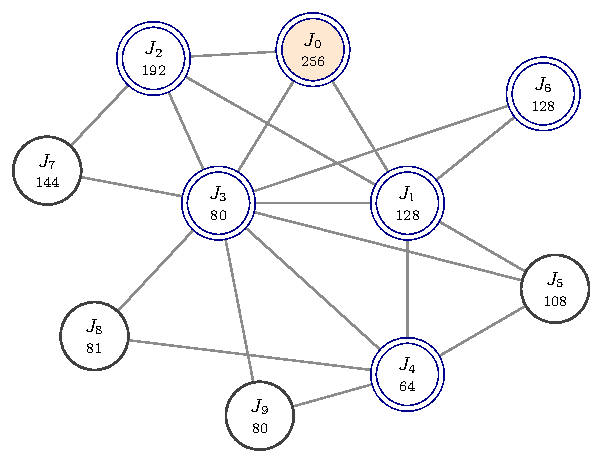
\includegraphics[width=0.74\textwidth]{figures/graph}
\caption{The ten classes of vertices of $\Rk$, labelled with $\det Q$, and the edges between different classes (Table~\ref{tab:edges}). The classes of $J_1$, $J_3$ and $J_4$ also have edges joining two vertices of the same class. Double circles mark the classes with unbounded edges. The packings of maximal density are the vertex $J_0$ and a point on an unbounded edge at $J_1$.}
\label{fig:graph}
\end{figure}

\appendix

\section{Computation and verification}\label{app:verification}

The computation behind Proposition~\ref{prop:computation} follows~\cite{AK2020} and Voronoi's algorithm~\cite{Voronoi1908,Schuermann2009}, in exact arithmetic throughout. All files are archived with the paper~\cite{Bhattacharjee2026}; the script \nolinkurl{verification/shell/run_all.sh} runs every check. The author used Claude (Anthropic), an AI system, for programming, computation and drafting; the author checked the mathematics and is responsible for the content.

\subsection*{Enumeration} Starting from $J_0$, for each new vertex $J$ the program \texttt{ryshkov2.py} (Python, rational arithmetic) computes $\Min(J)$ by the enumeration method of Fincke and Pohst, applied to the forms of Lemma~\ref{lem:sigma}(1) with rational bounds for the square roots; computes the extreme rays of $C_J$ with \texttt{cddlib} in GMP rational arithmetic; for each ray $Y$ decides whether $t^*=\infty$ and otherwise finds $t^*$ exactly (by the sign pattern of $Q(Y)$, a unimodular reduction of its kernel, and a descent through crossing points $t=(J[k]-4)/(-Y[k])$); and tests $\Gamma$-equivalence of $J+t^*Y$ with the known vertices by a backtracking search over images of minimal vectors. The search closes after ten classes and $1137$ rays, and \texttt{certify.py} writes the certificates of Proposition~\ref{prop:computation} as integer tables.

\subsection*{Independent checks}
\begin{enumerate}
\item \textbf{C} (\texttt{check\_polyhedron.c}, integers with overflow traps): recomputes $\Min(J_i)$ and checks $\min_{\M^*}J_i=4$ and rank $15$; recomputes all extreme rays of each $C_{J_i}$ from all $14$-element subsets of $\Min(J_i)$, independently of \texttt{cddlib}, and compares them with the list; for every bounded edge checks $\min_{\M^*}(J_i+t^*Y)=4$, rank $15$, $T\in\Gamma$ and $T^{\mathsf T}J_jT=J_i+t^*Y$; for every unbounded edge checks $Y=X_{u,a}$.
\item \textbf{Julia} (\texttt{check\_candidates.jl}, rational arithmetic): without using the concavity argument of Proposition~\ref{prop:candidates}, isolates with Sturm sequences all roots of $\det(J_i+tY)$ in $(0,t^*)$ on all $1137$ edges, decides the sign of $\det Q-256$ at each, and checks that the points with $\det Q=256$ are $J_0$ and the point $J_1+2X_{e_1,-1}$ (up to the orbit). It finds $21$ edge points, as in Table~\ref{tab:unbounded}.
\item \textbf{Lean~4} (\texttt{R4Check.lean}): proves the integer inequality of Lemma~\ref{lem:Xua} in the kernel, and checks by evaluation the invariants of Table~\ref{tab:vertices}, the minimal vectors, the $1112$ relations $T^{\mathsf T}J_jT=J_i+t^*Y$ with $T\in\Gamma$, the $25$ identities $Y=X_{u,a}$, and the orbit decomposition of the unbounded edges in Table~\ref{tab:unbounded}.
\item \textbf{Python} (\texttt{edges.py}, \texttt{sympy}): repeats the candidate analysis of the Julia check with exact real-root isolation.
\end{enumerate}
Floating-point numbers appear only in the C program, to choose enumeration boxes, which are widened by two units in every coordinate; every decision is made in integer arithmetic. The Gram determinants $144+64\sqrt5$ and $320$ of the non-maximal candidates agree with the densities $2/\sqrt{144+64\sqrt5}$ and $1/(4\sqrt5)$ reported in~\cite[\S4.2]{AK2020}.

\section*{Statements and Declarations}

\subsection*{Funding} No funding was received for conducting this study.

\subsection*{Competing interests} The author has no competing interests to declare that are relevant to the content of this article.

\subsection*{Data and code availability} The code, the data and the certificates of Appendix~\ref{app:verification} are available at \url{https://github.com/creelie/eD424} and are archived on Zenodo~\cite{Bhattacharjee2026}.

{\raggedright
\begin{thebibliography}{99}

\bibitem{AK2020}
A.~Andreanov and Y.~Kallus, \emph{Locally optimal 2-periodic sphere packings}, Discrete Comput. Geom. \textbf{63} (2020), 182--208. \doi{10.1007/s00454-019-00150-6}

\bibitem{Bhattacharjee2026}
D.~Bhattacharjee, \emph{Densest packings of two translates of a lattice in four dimensions: paper, code and certificates}, Zenodo, 2026. \doi{10.5281/zenodo.23239767}

\bibitem{Cassels1959}
J.~W.~S. Cassels, \emph{An Introduction to the Geometry of Numbers}, Grundlehren Math. Wiss. 99, Springer, Berlin, 1959. \doi{10.1007/978-3-642-62035-5}

\bibitem{CS1999}
J.~H. Conway and N.~J.~A. Sloane, \emph{Sphere Packings, Lattices and Groups}, 3rd ed., Grundlehren Math. Wiss. 290, Springer, New York, 1999. \doi{10.1007/978-1-4757-6568-7}

\bibitem{KZ1877}
A.~Korkine and G.~Zolotareff, \emph{Sur les formes quadratiques positives}, Math. Ann. \textbf{11} (1877), 242--292. \doi{10.1007/BF01442667}

\bibitem{Musin2018}
O.~R. Musin, \emph{Towards a proof of the 24-cell conjecture}, Acta Math. Hungar. \textbf{155} (2018), 184--199. \doi{10.1007/s10474-018-0828-5}

\bibitem{Schuermann2009}
A.~Sch\"urmann, \emph{Computational Geometry of Positive Definite Quadratic Forms}, Univ. Lecture Ser. 48, Amer. Math. Soc., Providence, RI, 2009. \doi{10.1090/ulect/048}

\bibitem{Voronoi1908}
G.~Voronoi, \emph{Nouvelles applications des param\`etres continus \`a la th\'eorie des formes quadratiques. Premier m\'emoire. Sur quelques propri\'et\'es des formes quadratiques positives parfaites}, J. Reine Angew. Math. \textbf{133} (1908), 97--178. \doi{10.1515/crll.1908.133.97}

\bibitem{Ziegler1995}
G.~M. Ziegler, \emph{Lectures on Polytopes}, Grad. Texts in Math. 152, Springer, New York, 1995. \doi{10.1007/978-1-4613-8431-1}

\end{thebibliography}
}

\end{document}
